\title{Study Guide for Midterm 2 for Calculus-Based Physics: Electricity and Magnetism}
\author{Dr. Jordan Hanson - Whittier College Dept. of Physics and Astronomy}
\date{\today}
\documentclass[10pt]{article}
\usepackage[a4paper, total={18cm, 27cm}]{geometry}
\usepackage{outlines}
\usepackage{graphicx}
\begin{document}
\maketitle

\begin{enumerate}
\item \textbf{Chapter 21: DC Circuits and Kirchhoff's Rules}
\begin{enumerate}
\item 
\begin{figure}[ht]
\centering
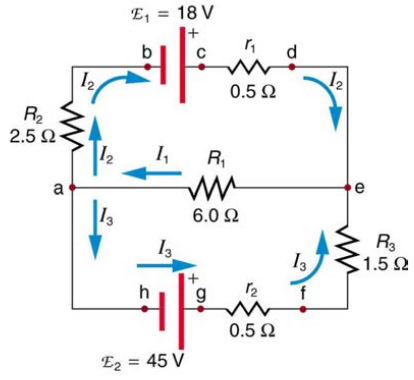
\includegraphics[width=0.4\textwidth]{circuit1.png}
\caption{\label{fig:circuit1} A circuit with five resistors (two are internal to the two batteries).}
\end{figure}
Solve for the currents $I_1$-$I_3$ in Fig. \ref{fig:circuit1}.  What is the total power consumption? \\ \vspace{4cm}
\item 
\begin{figure}[ht]
\centering
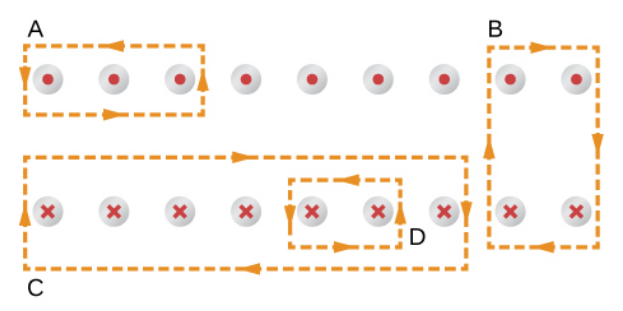
\includegraphics[width=0.4\textwidth]{circuit2.png}
\caption{\label{fig:circuit2} A circuit consisting of two batteries and five resistors.}
\end{figure}
Solve algebraiclly for the five currents in Fig. \ref{fig:circuit2}.  Remember to use the \textit{junction rule} and the \textit{loop rule.} \\ \vspace{4cm}
\item A person with body resistance between his hands of 10.0 k$\Omega$ accidentally grasps the terminals of a 20.0 kV power supply. (Do NOT do this!) (a) Draw a circuit diagram to represent the situation. (b) If the internal resistance of the power supply is 2000 $\Omega$, what is the current through his body? (c) What is the power dissipated in his body? (d) If the power supply is to be made safe by increasing its internal resistance, what should the internal resistance be for the maximum current in this situation to be 1.00 mA or less? \\ \vspace{3cm}
\end{enumerate}
\item \textbf{Chapter 22: Magnetic fields}
\begin{enumerate}
\item What Hall voltage is produced by a 0.200-T field applied across a 2.60-cm-diameter aorta when blood velocity is 60.0 cm/s? \\ \vspace{2cm}
\item Calculate the Hall voltage induced on a patient’s heart while being scanned by an MRI unit. Approximate the conducting path on the heart wall by a wire 7.50 cm long that moves at 10.0 cm/s perpendicular to a 1.50-T magnetic field. \\ \vspace{2cm}
\item (a) An oxygen-16 ion with a mass of $2.66\times 10^{−26}$ kg travels at $5.00 \times 10^{6}$ m/s perpendicular to a 1.20-T magnetic field, which makes it move in a circular arc with a 0.231-m radius. What positive charge is on the ion? (b) What is the ratio of this charge to the charge of an electron? (c) Discuss why the ratio found in (b) should be an integer. \\ \vspace{2cm}
\item 
\begin{figure}[ht]
\centering
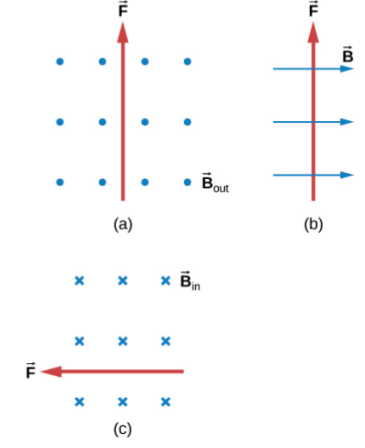
\includegraphics[width=0.3\textwidth]{lorentz1.png}
\caption{\label{fig:lorentz1} Each diagram depicts the force on a negatively-charged particle in a B-field.}
\end{figure}
Determine the velocity of a negatively-charged particle in Fig. \ref{fig:lorentz1} (a)-(c). \\ \vspace{1cm}
\item A cosmic-ray electron moves at $6 \times 10^6$ m/s perpendicular to Earth’s magnetic field at an altitude where the field strength is $1.0 \times 10^{-5}$ T. What is the radius of the circular path the electron follows?  Show that the \textit{angular velocity} $\omega$ of the electron around the magnetic field lines is related to the $q/m$ ratio by $\omega/B = q/m$. \\ \vspace{1.5 cm}
\item What is the (a) maximum torque on a 150-turn circular loop of wire with radius 8.0 cm that carries a 50.0-A current in a 1.60 T B-field? (b) What is the magnetic moment of this object? \\ \vspace{2 cm}
\item Using one of the results of Amp\`{e}re's Law, what is the magnetic field created by the loops in the previous problem, at the center of the loops? \\ \vspace{2cm}
\item Model a lightning bolt as a long straight wire.  A typical current in a lightning bolt is $10^4$ A. Estimate the magnetic field 1 m from the bolt, using one of the results of Amp\`{e}re's Law. \\ \vspace{2cm}
\item 
\begin{figure}[hb]
\centering
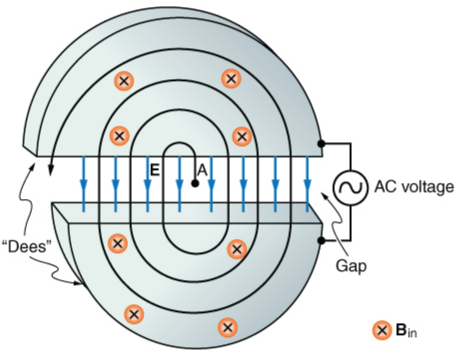
\includegraphics[width=0.35\textwidth]{cyclo.png}
\caption{\label{fig:cyclo} Each diagram depicts the force on a negatively-charged particle in a B-field.}
\end{figure}
(a) Show that the period $T$ of the circular orbit of a charged particle with mass $m$ and charge $q$ moving perpendicularly to a uniform magnetic field is $T = 2\pi m/(qB)$. (b) What is the frequency $f$? (c) What is the angular velocity $\omega$?  (c) A cyclotron accelerates charged particles as shown in Fig. \ref{fig:cyclo}. Calculate the frequency of the accelerating voltage needed for a proton in a 0.9 T B-field.
\end{enumerate}
\end{enumerate}
\end{document}